%===================================== CHAP 5 =================================

\chapter{Evaluation and Testing Methodology}
\label{sec:eval}
This chapter covers the methodology used for evaluating the detection algorithms used, as well as the dataset used for testing. The goal of this chapter is to show how the two detection algorithms have been tested, and how they can be compared using the measures explained.

\section{Precision and Recall}
\label{sec:prec_rec}

Two common performance measures used in object detection are \textit{precision} and \textit{recall}. By using these two measures, both the false negatives and the false positives are taken into account. Recall measures how many of the true positives in the image are detected and precision measures how many of the detections that are correct. This is also shown graphically in figure \ref{fig:prec_recall}. In detection, theory recall is often referred to as \textit{probability of detection}. A high precision would correspond to what detection theory calls a low \textit{false alarm rate}.

\begin{figure}[h!]
    \centering
    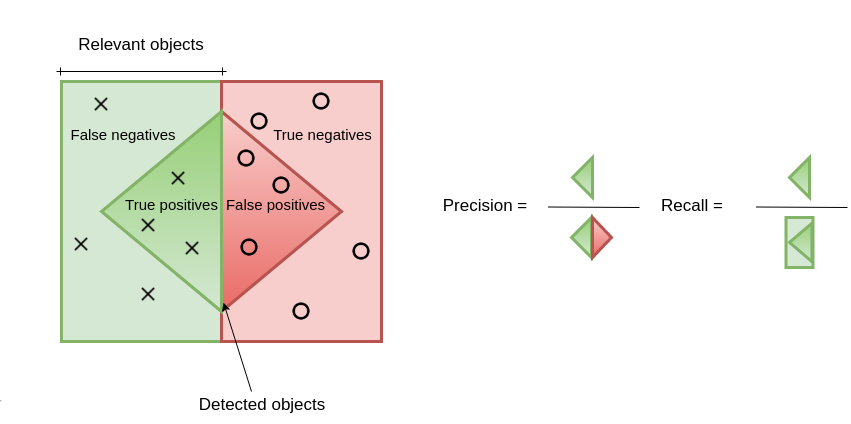
\includegraphics[scale=0.33]{fig/recall_precision.png}
    \caption{Precision and recall}
    \label{fig:prec_recall}
\end{figure}


\newpage

\section{Bounding Box Evaluation}
To be able to calculate the precision and recall, there must be a definition of what a correct detection is. In \citep{Everinghama} this is defined the following way: "Detections are considered true or false positives based on the area of overlap
with ground truth bounding boxes. To be considered a correct detection, the area of overlap $a_0$ between the predicted bounding box $B_p$ and ground truth bounding box $B_{gt}$ must exceed 50\% by the formula:"

\begin{equation*}
    a_0 = \frac{area(B_p \cap B_{gt}) }{area(B_p \cup B_{gt})}
\end{equation*}

The area of overlap is the same as intersect over union explained in figure \ref{fig:IoU}. The same definition is used in this report.




\section{Precision/Recall Curves}

In the VOC challenge \citep{Everinghama} the detection task is judged by a precision/recall curve. The precision/recall curve is made by checking the precision and recall for the detection algorithm at different confidence score thresholds. The confidence score used is the score returned from the detection algorithms along with the bounding box, i.e., how confident the algorithm is in the bounding box. If the confidence score threshold is low, the detection algorithm will likely detect more objects of interest, but also identify more false positives. This means that for a low confidence score threshold the recall will be high and the precision low. In figure \ref{fig:yolo_prec_recall} an example of a precision/recall curve is shown, and the results in this report will be presented in the same manner. 

\vspace{3mm}

We want both the recall and the precision to be as high as possible, meaning that in the precision/recall curve we would like to get as far up in the top right corner as possible. As shown in figure \ref{fig:yolo_prec_recall}, the precision decreases while the recall increases. This is the expected behavior since more boats are detected when the threshold based on the confidence score is lowered. More detections also increase the number of false negatives. Sometimes it can be hard to decide precisely what the optimal confidence score threshold should be, since this is a trade-off between recall and precision and will be discussed further in the next chapter. 

\begin{figure}[h!]
    \centering
    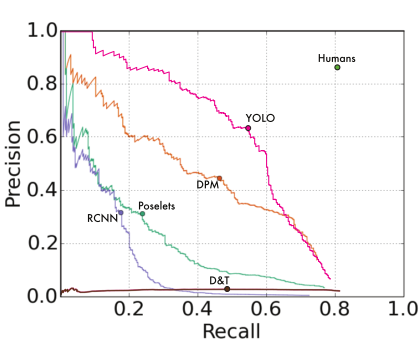
\includegraphics[scale=0.4]{fig/yolo_prec_recall.png} 
    \caption{Precision/recall curve from \citep{YOLOv1}}
    \label{fig:yolo_prec_recall}
\end{figure}

\section{Average precision}
Average precision (AP) is a commonly used metric in object detection and is used in the papers of, e.g. Faster R-CNN, YOLO, and SSD. It is the average of the maximum precision at different recall levels.

\begin{equation}
    AP = \frac{1}{11} \Sigma_{r \in \{0.0, ... , 1.0\}} p_{interp}(r)
\end{equation}

Where
\begin{equation}
    p_{interp}(r) = max_{\tilde{r} \geq r} p(\tilde{r})
\end{equation}

Meaning that for each recall value in {0.0, ... , 1.0} the highest precision level at that recall level, or a higher recall level, is added to the sum. This is illustrated in figure \ref{fig:p_interp}, where the green line shows $p_{interp}(r)$

\begin{figure}[h!]
    \centering
    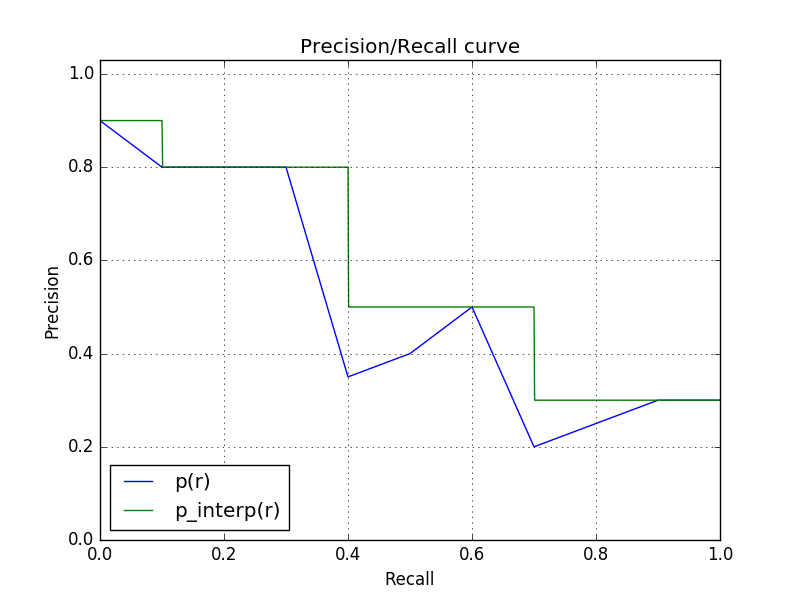
\includegraphics[scale=0.5]{fig/p_interp.png}
    \caption{$p(r) and p_{interp}(r)$}
    \label{fig:p_interp}
\end{figure}

\section{Confusion Matrix}
\label{sec:conf_mat}
A confusion matrix is another way of presenting the performance of a classification algorithm. The confusion matrix gives a more intuitive representation of the results, and gives a clearer indication on how well the detection algorithm would work in a real scenario. In this project the goal is to identify boats, thus it is a two-class problem with boat and not-boat as the two classes. 

\begin{figure}[h!]
    \centering
    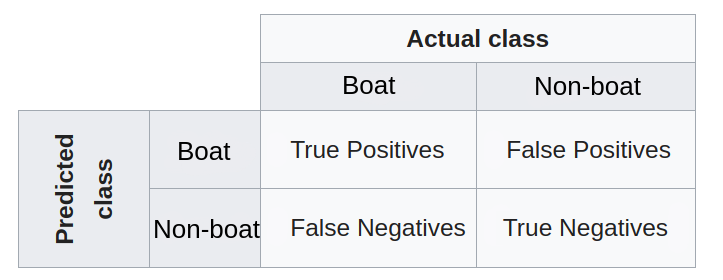
\includegraphics[width = 0.7 \textwidth]{fig/conf_e.png}
    \caption{Confidence matrix}
    \label{fig:conf_exp}
\end{figure}

\newpage

Table \ref{fig:conf_exp} shows how the confusion matrix will be used in this project. True positives are boats detected correctly, false positives are detections that are uncorrect, false negatives are undetected boats. The detections algorithms developed in this project does not seek to identify non-boat objects, rather to overlook them, thus true negatives cannot be quantized and are not relevant in this work.






\cleardoublepage